
\documentclass[fleqn,addpoints]{exam}

\usepackage{units} 
\usepackage{graphicx}
\usepackage[fleqn]{amsmath}
\usepackage{cancel}
\usepackage{float}
\usepackage{mdwlist}
\usepackage{booktabs}
\usepackage{cancel}
\usepackage{polynom}
\usepackage{caption}
\usepackage{fullpage}
\usepackage{xfrac}
\usepackage{enumerate}

\everymath{\displaystyle}

% \printanswers

\ifprintanswers
  \usepackage{2in1, lscape}
\fi

\title{Math 141 Chapter Four Exam}
\date{July 17, 2013}
\author{}

\begin{document}

  \maketitle  

  % \ifprintanswers
  %   \else
  %   \vspace{0.2in}
  %   \makebox[\textwidth]{Name:\enspace\hrulefill}
  %   \vspace{0.2in}

  %   \begin{center}
  %   \gradetable[h][pages]
  %   \bonusgradetable[h][pages]
  %   \end{center}
  % \fi

  % \vspace{1 cm}

  % \ifprintanswers
  % \else
  %   \pagebreak
  % \fi

  \begin{questions}
    \uplevel{\section{Questions}}

    \question Write in logarithm form
      \begin{parts}
        \part[2] $2^3 = 8$

        \part[2] $e^x = y$
      \end{parts}

    \question Write in exponential form
      \begin{parts}
        \part[2] $\log_3 81 = 4$

        \part[2] $\ln x = 5$
      \end{parts}

    \question Evaluate each expression.
      \begin{parts}

        \part[2] $\log_8 64$

        \part[2] $\log 0.001$

        \part[2] $\log_7 \frac{1}{49}$

        \part[2] $\log_9 27$

        \part[2] $\log_8 16 + \log_8 32$

        \part[2] $\log_5 100 - \log_5 4$

      \end{parts}

      \question solve for x:
      \[
        \log_x 27 = \frac{3}{2}
      \]

    \question $f(x) = 1 - 2^x$
      \begin{parts}
        \part[3] what is the range?

        \part[2] what is the y-intercept?

        \part[5] plot the graph
          \begin{solution}
            \begin{figure}[H]
              \centering
              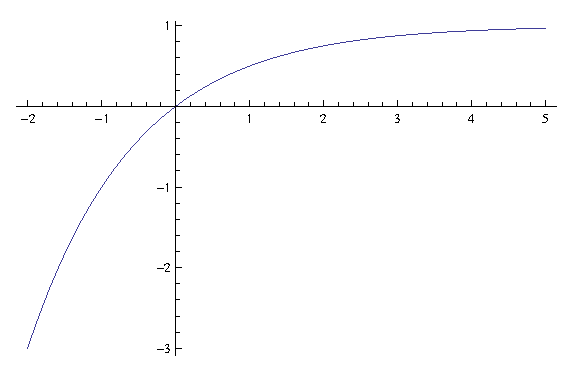
\includegraphics[scale=0.9]{graph_1.eps}
              \caption*{$f(x) = 1 - 2^x$}
            \end{figure}
          \end{solution}

      \end{parts}

    \question $f(x) = 3^{-x} + 2$
      \begin{parts}
        \part[3] what is the range?

        \part[2] what is the y-intercept?

        \part[5] plot the graph
          \begin{solution}
            \begin{figure}[H]
              \centering
              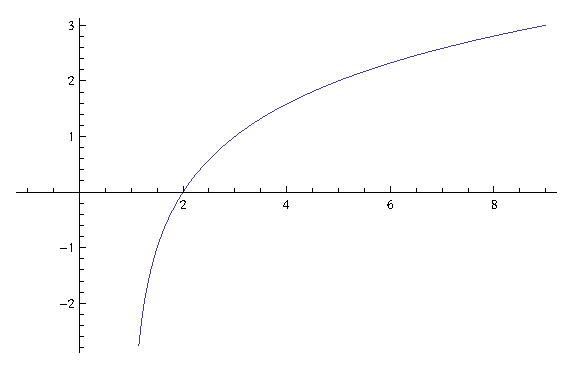
\includegraphics[scale=0.9]{graph_2.eps}
              \caption*{$f(x) = 3^{-x} + 2$}
            \end{figure}
          \end{solution}
      \end{parts}

      \uplevel{\section{Extra Credit}}

      \bonusquestion[10]
        Multiply three consecutive integers together and then add the second integer to the product.  Use synthetic
        division to help prove that the sum is the cube of an integer and determine which integer.

        \begin{solution}
          If $x$ is the first number, the other two numbers are $x + 1$ and $x + 2$.  When you multiply the three
          numbers and add the second one, you get:
          \[
            x(x + 1)(x + 2) + (x + 1) = x^3 + 3x^2 + 3x + 1
          \]

          The only possible zeros are $x = \pm 1$.  If you try both of them, you find that $(x + 1)$ is the only
          factor and:
          \[
            x^3 + 3x^2 + 3x + 1 = (x + 1)^3
          \]

          Another way of seeing the same thing without doing any division is to factor $(x+1)$ out of the original
          equation and simplify:
          \begin{align*}
            x(x + 1)(x + 2) + (x + 1) &= (x+1) [ x(x+2) + 1 ] \\
                                      &= (x + 1) \left( x^2 + 2x + 1 \right) \\
                                      &= (x + 1) (x + 1)^2 \\
                                      &= (x + 1)^3 \\
          \end{align*}
          
        \end{solution}
  \end{questions}

\end{document}

